\documentclass[a4paper,10pt]{book}

\usepackage[utf8]{inputenc}
\usepackage{color}
\usepackage{bm}
\usepackage{amsmath}
\usepackage{appendix}
\usepackage{xspace}
\usepackage{a4wide}
\usepackage{wrapfig}
\usepackage[numbers,comma,sort&compress]{natbib}
\usepackage{graphicx}
\usepackage{xstring}
\usepackage{listings,xcolor,courier}
%\usepackage{draftcopy}
\usepackage{longtable}
\usepackage{booktabs}
\usepackage{paralist}

\usepackage
[dvips, %or dvips or pdftex
pagebackref, %or backref
colorlinks=true,
linkcolor=webgreen, %defined below
filecolor=webbrown, %defined below
citecolor=webgreen, %defined below
pdftitle={VOTCA manual},
pdfauthor={},
pdfsubject={VOTCA},
pdfkeywords={coarse-graining boltzmann inversion monte carlo force matching},
bookmarksopen=false,
pdfpagemode=UseNone]{hyperref}

\definecolor{webgreen}{rgb}{0,.5,0}
\definecolor{webbrown}{rgb}{.6,0,0}
\pdfcompresslevel=9

\usepackage[T1]{fontenc}
%\usepackage{times}
\usepackage{type1cm}

\renewcommand{\vec}[1]{\ensuremath{{\bm #1}}}
\newcommand{\fig}[1]{fig.~\ref{#1}}
\newcommand{\eq}[1]{eq.~\ref{#1}}
\newcommand{\unit}[1]{\ensuremath{\,\mbox{#1}}}
\newcommand{\sign}{\ensuremath{\operatorname{sgn}}}
\newcommand{\ibi}{IBI\xspace}
\newcommand{\imc}{IMC\xspace}
\newcommand{\fm}{FM\xspace}
\newcommand{\xml}{XML\xspace}
\newcommand{\gromacs}{GROMACS\xspace}
\newcommand{\espresso}{ESPResSo\xspace}
\newcommand{\dlpoly}{DL\_POLY\xspace}
\newcommand{\dlpolyfour}{DL\_POLY-4\xspace}
\newcommand{\spce}{SPC/E\xspace}
\newcommand{\grad}{\vec{\nabla}}
\newcommand{\ddash}{{-}{-}\xspace}

%formating for a program option, e.g. --trj
\newcommand{\progopt}[1]{\texttt{#1}\xspace}
% formating for intern programs, e.g. csg_boltzmann
\newcommand{\prog}[1]{\hyperref[#1]{\textbf{\StrSubstitute{#1}{_}{\_}}}\xspace}
% formating for external programs, e.g. grompp
\newcommand{\progex}[1]{\hyperlink{progex.#1}{\textbf{#1}\xspace}}

% reference to an xml option in the reference section
\newcommand{\cgref}[1]{cg.#1}

%we need \StrSubstitute{#1}{_}{\_} to replace _ \_ in the text of the reference (not in the label it self)

%hyperlink for cgopts
\newcommand{\cgopt}[1]{\hyperlink{\cgref{#1}}{\textit{\StrSubstitute{#1}{_}{\_}}}\xspace}
\newcommand{\interref}[1]{cg.non-bonded.#1}
\newcommand{\interopt}[1]{\hyperlink{\interref{#1}}{\textit{\StrSubstitute{#1}{_}{\_}}}\xspace}
\newcommand{\mapref}[1]{cg_molecule.#1}
\newcommand{\mapopt}[1]{\hyperlink{\mapref{#1}}{\StrSubstitute{#1}{_}{\_}}\xspace}

\newcommand{\sect}[1]{sec.~\ref{#1}}

\newcommand{\votca}{{\sc \color{blue} votca}\xspace}
\newcommand{\votcaweb}{\htmladdnormallink{{\sc \color{blue} www.votca.org}\xspace}{http://www.votca.org}}

\input{hgid}
\input{reference/csgid}

% todo
\newcommand{\todo}{{\marginpar{\sc \color{red} TODO}}\xspace}

% XML listings
\definecolor{darkgreen}{named}{green}
\definecolor{darkblue}{named}{blue}
\definecolor{darkred}{named}{red}
\definecolor{grau}{named}{gray}
\let\Righttorque\relax

\lstset{language=XML}

\lstset{
    language=XML,
    basicstyle=\ttfamily,%\scriptsize\mdseries,
    keywordstyle=,
    identifierstyle=,
    commentstyle=\color{gray},
    stringstyle=\itshape\color{black},
    breaklines=true,
    frame=none,
    showstringspaces=false,
    tabsize=2,
    captionpos=b,
    float=htbp,
    moredelim=*[s][\color{darkblue}]{<}{>},
    morecomment=[s]{<!--}{-->},
}



\begin{document}
\frontmatter
\begin{titlepage}

\center{\fontsize{4cm}{5cm}\selectfont VOTCA}
\center{\fontsize{1.5cm}{3cm}\selectfont USER MANUAL}

\vspace*{3cm}
\center{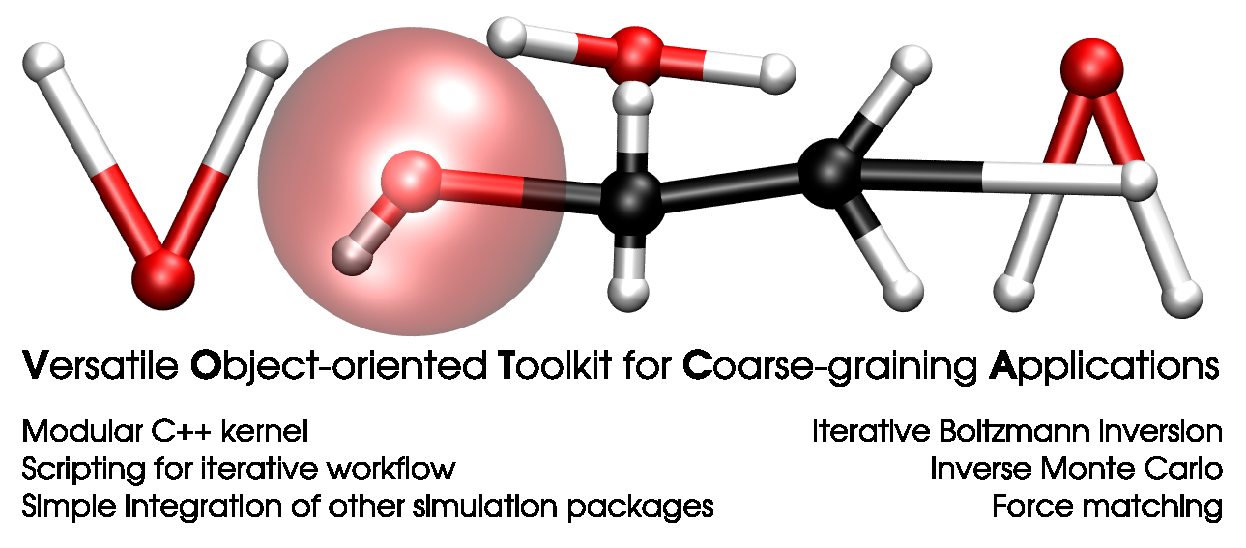
\includegraphics[width=\columnwidth]{fig/logo}}
\vspace*{1cm}
\vfill
\vspace*{1.4cm}
\center{\large{\today}}
\vspace*{-0.3cm}
\center{\footnotesize{Version: \gitid}}
\center{\footnotesize{Programs version: \csgid}}

\vspace*{1cm}
%\center{
\large{\copyright \hspace*{0.1cm} VOTCA development team}
%}
\vspace*{0.5cm}

\htmladdnormallink{\color{black}\large{www.votca.org}}{http://www.votca.org}
\end{titlepage}

\thispagestyle{empty}
\cleardoublepage

\tableofcontents
\cleardoublepage
\mainmatter
\chapter{Introduction}
\chapter{Theoretical background}

\section{Mapping}
\label{sec:mapping_operator}
%\sasha
%mapping scheme ($c_{Ii}$ coefficients) \\
%TO DO: picture \\
%translation invariance \\
%definition of the mass \\
%definition of specific and involved atoms \\

The mapping is an operator that establishes a link between the atomistic and coarse-grained representations of the system. An atomistic system is described by specifying the values of the Cartesian coordinates and momenta
\begin{eqnarray}
\bm r^n &=& \{\bm r_1,\dots,\bm r_n\}, \\
\bm p^n &=& \{\bm p_1,\dots,\bm p_n\}.
\end{eqnarray}
of the $n$ atoms in the system.\footnote{In what follows we adopt notations of ref.~\cite{Noid:2008.1}.}
%
On a coarse-grained level, the coordinates and momenta are specified by the positions and momenta of CG sites
\begin{eqnarray}
\bm R^N = \{\bm R_1,\dots,\bm R_N\}, \\
\bm P^N = \{\bm P_1,\dots,\bm P_N\}.
\end{eqnarray}
Note that capitalized symbols are used for the CG sites while lower case letters are used for the atomistic system.

The mapping operator ${\bm c}_I$ is defined by a matrix for each bead $I$ and links the two descriptions
\begin{eqnarray}
 {\bm R}_I &=& \sum_{i=1}^{n}c_{Ii}\bm r_i, \\
 {\bm P}_I &=&
 	M_I \dot{{\bm R}}_I =
	M_I \sum_{i=1}^{n}c_{Ii} \dot{{\bm r}}_i =
	M_I \sum_{i=1}^{n} \frac{ c_{Ii}} {m_i} {\bm p}_i .
\label{eq:mapping_scheme}
\end{eqnarray}
for all $I = 1,\dots,N$.

If an atomistic system is translated by a constant vector, the corresponding coarse-grained system is also translated by the same vector. This implies that, for all $I$,
\begin{equation}
 \sum_{i=1}^{n}c_{Ii}=1.
\end{equation}

In some cases it is useful to define the CG mapping in such a way that certain atoms belong to several CG beads at the same time~\cite{Fritz:2009}. Following ref.~\cite{Noid:2008.1}, we define two sets of atoms for each of the $N$ CG beads. For each site $I$, a set of {\em involved} atoms is defined as
\begin{equation}
 {\cal I}_I=\{i|c_{Ii}\ne0\}.
\end{equation}
An atom $i$ in the atomistic model is involved in a CG site, \textit{I}, if and only if this atom provides a nonzero contribution to the sum in eq.~\ref{eq:mapping_scheme}.

A set of {\em specific} atoms is defined as
\begin{equation}
 {\cal S}_I=\{i|c_{Ii}\ne0 \text{ and } c_{Ji}=0 \text{ for all } J \ne I\}.
\end{equation}
In other words, atom $i$ is specific to site $I$ if and only if this atom is involved in site $I$ and is not involved in the definition of any other site.

The CG model will generate an equilibrium distribution of momenta that is consistent with an underlying atomistic model if all the atoms are {\em specific} and if the mass of the $I^\text{th}$ CG site is given by~\cite{Noid:2008.1}
\begin{equation}
M_I= \left( \sum_{i \in {\cal I}_I}\frac{c_{Ii}^2}{m_i} \right)^{-1}.
\label{eq:cg_mass}
\end{equation}
%
If all atoms are specific and the center of mass of a bead is used for mapping, then $c_{Ii} = \frac{m_i}{M_I}$, and the condition~\ref{eq:cg_mass} is automatically satisfied.

%%%%%%%%%%%%%%%%%%%%%%%%%%%%%%%%%%%%%%%%%%%%%%%%%%%%%%%%%%%%%%%%%%%%%%%%%%%%%%%%%
\section{Boltzmann inversion}
\label{sec:bi}

Boltzmann inversion is mostly used for {\em bonded} potentials, such as bonds, angles, and torsions~\cite{Tschoep:1998}. Boltzmann inversion is structure-based and only requires positions of atoms.

The idea of Boltzmann inversion stems from the fact that in a canonical ensemble {\em independent} degrees of freedom $q$ obey the Boltzmann distribution, i.~e.
%
\begin{equation}
  P(q) = Z^{-1} \exp\left[ - \beta U(q) \right]~,
  \label{eq:boltzmann}
\end{equation}
%
where \mbox{$Z = \int \exp \left[ - \beta U(q) \right] \text{d}q $} is a partition function, \mbox{$\beta = 1/k_\text{B} T$}.
%
Once $P(q)$ is known, one can obtain the coarse-grained potential, which in this case is a potential of mean force, by inverting the probability distribution $P(q)$ of a variable $q$, which is either a bond length, bond angle, or torsion angle
\begin{equation}
  U(q) = - k_\text{B} T \ln  P(q) ~.
  \label{eq:inv_boltzmann}
\end{equation}
%
The normalization factor $Z$ is not important since it would only enter the coarse-grained potential $U(q)$ as an irrelevant additive constant.

Note that the histograms for the bonds $H_r(r)$, angles $H_\theta(\theta)$, and torsion angles $H_\varphi(\varphi)$ have to be rescaled in order to obtain the volume normalized distribution functions $P_r(r)$, $P_\theta(\theta)$, and $P_\varphi(\varphi)$, respectively,
%
\begin{align}
    P_r(r) = \frac{H_r(r)}{4\pi r^2}~,\;
    P_\theta(\theta) = \frac{H_\theta(\theta)}{\sin \theta}~,\;
    P_\varphi(\varphi) = H_\varphi (\varphi)~,
    \label{eq:boltzmann_norm}
\end{align}
where $r$ is the bond length $r$, $\theta$ is the bond angle, and $\varphi$ is the torsion angle. The bonded coarse-grained potential can then be written as a sum of distribution functions
%
\begin{align}
    \label{eq:boltzmann_pmf}
    U({r}, \theta, \varphi) &= U_r({r}) + U_{\theta}(\theta) + U_{\varphi}(\varphi)~, \\
    U_q({q}) &= - k_\text{B} T \ln P_q( q ),\; q=r, \theta, \varphi~.
    \nonumber
\end{align}

On the technical side, the implementation of the Boltzmann inversion method requires {\em smoothing} of $U(q)$ to provide a continuous force. Splines can be used for this purpose. Poorly and unsampled regions, that is regions with high $U(q)$, shall be {\em extrapolated}. Since the contribution of these regions to the canonical density of states is small, the exact shape of the extrapolation is less important.

Another crucial issue is the cross-correlation of the coarse-grained degrees of freedom. Independence of the coarse-grained degrees of freedom is the main assumption that allows factorization of the probability distribution and the potential, eq.~\ref{eq:boltzmann_pmf}. Hence, one has to carefully check whether this assumption holds in practice. This can be done by performing coarse-grained simulations and comparing cross-correlations for all pairs of degrees of freedom in atomistic and coarse-grained resolution, e.~g. using a two-dimensional histogram, analogous to a Ramachandran plot.~\footnote{Checking the linear correlation coefficient does not guarantee statistical independence of variables, for example $c(x, x^2)=0$ if $x$ has a symmetric probability density $P(x) = P(-x)$. This case is often encountered in systems used for coarse-graining.}

\subsection{Separation of bonded and non-bonded degrees of freedom}
When coarse-graining polymeric systems, it is convenient to treat bonded and non-bonded interactions separately~\cite{Tschoep:1998}. In this case, sampling of the atomistic system shall be performed on a special system where non-bonded interactions are artificially removed, so that the non-bonded interactions in the reference system do not contribute to the bonded interactions of the coarse-grained model.

This can be done by employing exclusion lists using \prog{csg_boltzmann} with the option \progopt{---excl}. This is described in detail in sec. \ref{sec:exclusions}.
\begin{figure}[h]
  \centering
  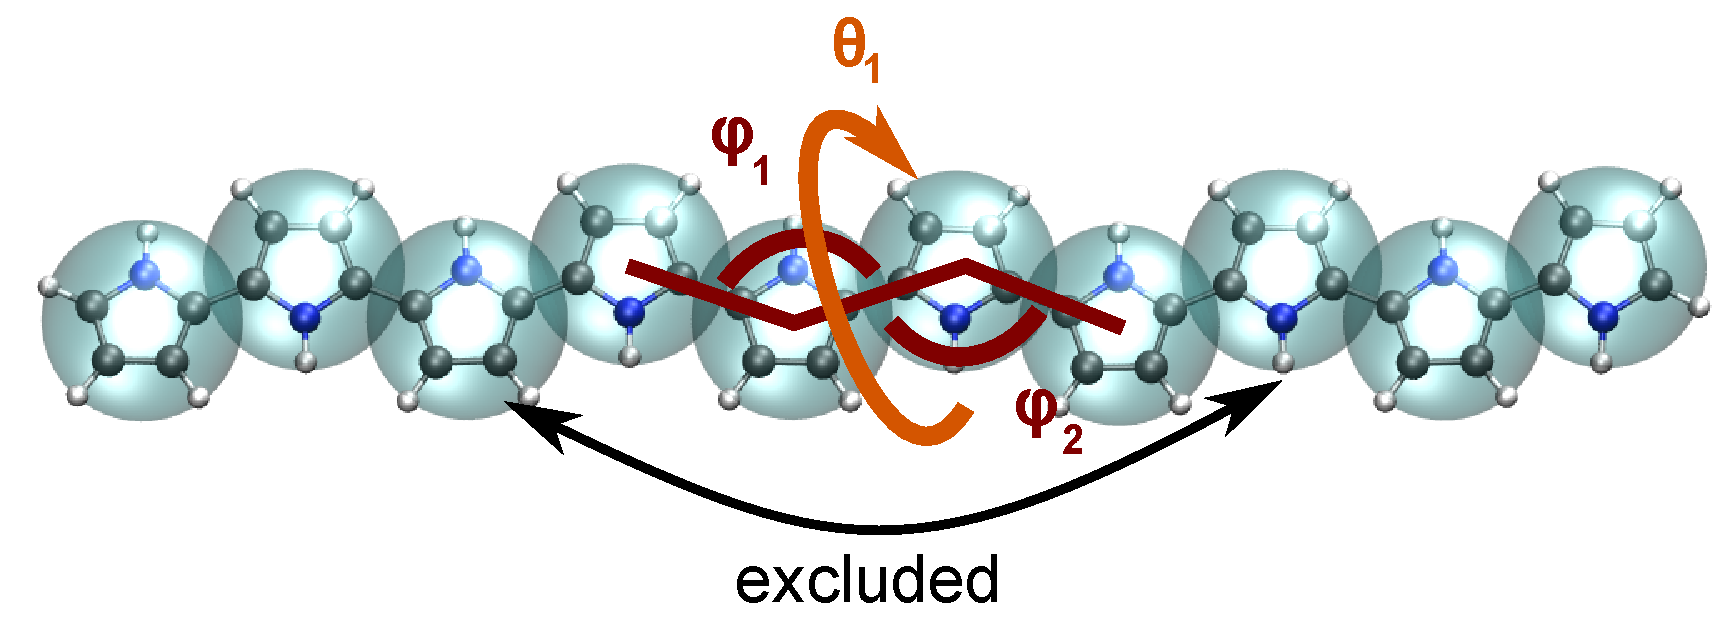
\includegraphics[width=0.7\textwidth]{fig/excl}
  \caption{\label{fig:excl}Example of excluded interactions.}
\end{figure}


%%%%%%%%%%%%%%%%%%%%%%%%%%%%%%%%%%%%%%%%%%%%%%%%%%%%%%%%%%%%%%%%%%%%%%%%%%%%%%%%%%%%%%%%%%%%%%%%
\newpage
\section{Iterative methods}
\label{sec:theory_iterative_methods}

\begin{wrapfigure}{ht}{3cm}  
%\includegraphics[width=3cm]{functionality/fig/iterativemethods.eps}
  \caption{
    \label{fig:iterative_methods}
    Block-scheme of an iterative method.
  }
\end{wrapfigure}
%\end{figure}
Iterative workflow control is essential for the \ibi and \imc methods. The general idea of iterative workflow is sketched in fig.~\ref{fig:iterative_methods}. A run starts with an initial guess during the global initialization phase. This guess is used for the first sampling step, followed by an update of the potential. The update itself often requires additional postprocessing such as smoothing, interpolation, extrapolation or fitting. Different methods are available to update the potential, for instance Iterative Boltzmann Inversion (see next section \ref{sec:ibi}) or Inverse Monte Carlo (see section \ref{sec:imc}). The whole procedure is then iterated until a convergence criterion is satisfied.


%%%%%%%%%%%%%%%%%%%%%%%%%%%%%%%%%%%%%%%%%%%%%%%%%%%%%%%%%%%%%%%%%%%%%%%%%%%%%%%%%%%%%%%%%%%%%%%%
\section{Iterative Boltzmann Inversion}
\label{sec:ibi}

Iterative Boltzmann inversion (\ibi) is a natural extension of the Boltzmann inversion method. Since the goal of the coarse-grained model is to reproduce the distribution functions of the reference system as accurately as possible, one can also iteratively refine the coarse-grained potentials using some numerical scheme.

In \ibi the potential update $\Delta U$ is given by~\cite{Reith:2003}
\begin{eqnarray}
  \label{eq:iter_boltzmann}
  U^{(n+1)} &=& U^{(n)} + \lambda \Delta U^{(n)}~, \\
  \Delta U^{(n)} &=&  k_\text{B} T \ln  \frac{P^{(n)}}{P_{\rm ref}}
  =  U_\text{PMF}^\text{ref} - U_\text{PMF}^{(n)}~.
\end{eqnarray}
Here $\lambda \in (0,1]$ is a numerical factor which helps to stabilize the scheme.

The convergence is reached as soon as the distribution function $P^{(n)}$ matches the reference distribution function $P_{\rm ref}$, or, in other words, the potential of mean force, $U_\text{PMF}^{(n)}$, converges to the reference potential of mean force.

\ibi can be used to refine both bonded and non-bonded potentials. It is primarily used for simple fluids with the aim to reproduce the radial distribution function of the reference system in order to obtain non-bonded interactions. On the implementation side, \ibi has the same issues as the inverse Boltzmann method, i.~e. smoothing and extrapolation of the potential must be used.


\section{Inverse Monte Carlo}
\label{sec:imc}

Inverse Monte Carlo (\imc) is an iterative scheme which additionally includes cross correlations of distributions. A detailed derivation of the \imc method can be found in ref.~\cite{Lyubartsev:1995}.

The potential update $\Delta U$ of the \imc method is calculated by solving a set of linear equations
\begin{align}
    \left<S_{\alpha}\right> - S_{\alpha}^{\text{ref}}= A_{\alpha \gamma} \Delta U_{\gamma}~,
  \label{eq:imc}
\end{align}
%
where
\begin{eqnarray}
  \label{eq:covariance}
  A_{\alpha \gamma} = \frac{\partial \left< S_{\alpha} \right> }{\partial U_{\gamma}}  =
  \beta \left( \left<S_{\alpha} \right>\left<S_{\gamma} \right> - \left<S_{\alpha} S_{\gamma} \right>  \right)~,
  \nonumber
\end{eqnarray}
and $S$ the histogram of a coarse-grained variable of interest. For example, in case of coarse-graining of the non-bonded interactions which depend only on the distance $r_{ij}$ between particles $i$ and $j$ and assuming that the interaction potential is short-ranged, i.e. $U(r_{ij})=0$ if $r_{ij} \ge r_{\text{cut} }$, the average value of $S_{\alpha}$ is related to the radial distribution function $g(r_{\alpha})$ by
%
\begin{equation}
   \left< S_{\alpha} \right> =  \frac{N(N-1)}{2} \frac{4 \pi r_{\alpha}^2 \Delta r} {V}g(r_{\alpha})~,
  \label{eq:s_mean}
\end{equation}
%
where $N$ is the number of atoms in the system ($\frac{1}{2} N(N-1)$ is then the number of all pairs), $\Delta r$ is the grid spacing, $r_{\text{cut}}/M$, $V$ is the total volume of the system. In other words, in this particular case the physical meaning of $S_{\alpha}$ is the number of particle pairs with interparticle distances $r_{ij} = r_{\alpha}$ which correspond to the tabulated value of the potential $U_{\alpha}$.

\subsection{Regularization of Inverse Monte Carlo}

To get a well defined cross correlation matrix, $A_{\alpha \gamma}$, enough sampling is needed. If there is not enough smapling or the initial potential guess is far from the real solution of the inverse problem, the algorithm might not converge to a stable solution. To overcome this instability problem one could reformulate equation \ref{eq:covariance} by addition of a penalty term. In this case the potential update is computed  as follows:\cite{Murtola:2007}
\begin{equation}
\label{eq:regularization}
\Delta U_\gamma = \arg \min \| A_{\alpha \gamma} \Delta U_\gamma - \left(\left<S_{\alpha}\right> - S_{\alpha}^{\text{ref}}\right) \|^2 + \lambda \| R \Delta U_{\gamma} \|^{2}
\end{equation}
%
Equation \ref{eq:regularization} is known as Tikhonov regularization,
where $R$ is the regularization operator, which here is the identity matrix and $\lambda >0 $ is the regularization parameter.
The optimal choice for $\lambda$ can only be determined if the exact solution of the inverse problem is known, which in practice is not the case. To get a good initial guess on the magnitude of the regularization parameter a singular value decomposition of the matrix $A_{\alpha \gamma}$ might help. A good $\lambda$ parameter should dominate the smallest singular values (squared) but is itself small compared to the larger ones.\cite{Rosenberger:2016}
 
\section{Force Matching}
\label{sec:fm}

%\sasha

%Brief description with references \\
% Maybe appendix with main equations \\

Force matching (\fm) is another approach to evaluate corse-grained potentials~\cite{Ercolessi:1994,Izvekov:2005,Noid:2007}. In contrast to the structure-based approaches, its aim is not to reproduce various distribution functions, but instead to match the multibody potential of mean force as close as possible with a given set of coarse-grained interactions.

The method works as follows. We first assume that the coarse-grained force-field (and hence the forces) depends on $M$ parameters $g_1,...,g_M $. These parameters can be prefactors of analytical functions, tabulated values of the interaction potentials, or coefficients of splines used to describe these potentials.

In order to determine these parameters, the reference forces on coarse-grained beads are calculated by summing up the forces on the atoms
\begin{equation}
  {\vec F}_I^\text{ref} = \sum_{j \in {\cal S_I}} \frac{d_{Ii}}{c_{Ii}} {\vec f}_j({\vec r^n}),
  \label{eq:force_mapping}
\end{equation}
where the sum is over all atoms of the CG site {\it I} (see. \sect{sec:mapping_operator}).
The $d_{Ij}$ coefficients can, in principle, be chosen arbitrarily, provided that the condition $ \sum_{i=1}^{n}d_{Ii}=1$ is satisfied~\cite{Noid:2008.1}. If mapping coefficients for the forces are not provided, it is assumed that $d_{Ij} = c_{Ij}$ (see also \sect{sec:inputfiles}).

By calculating the reference forces for $L$ snapshots we can write down $N \times L$ equations
%
\begin{equation}
  {\vec F}_{Il}^\text{cg}(g_1, \dots ,g_M)=\vec F_{il}^\text{ref},\;
  I=1,\dots,N,\; l=1,\dots,L~.
  \label{eq:fmatch1}
\end{equation}
%
Here ${\vec F}_{Il}^\text{ref}$ is the force on the bead $I$ and ${\vec F}_{Il}^\text{cg} $ is the coarse-grained representation of this force. The index $l$ enumerates snapshots picked for coarse-graining. By running the simulations long enough one can always ensure that $M < N \times L$. In this case the set of equations~\ref{eq:fmatch1} is overdetermined and can be solved in a least-squares manner.

${\bm F}_{il}^\text{cg}$ is, in principle, a non-linear function of its parameters $\{g_i\}$. Therefore, it is useful to represent the coarse-grained force-field in such a way that equations~(\ref{eq:fmatch1}) become linear functions of $\{g_i\}$. This can be done using splines to describe the functional form of the forces~\cite{Izvekov:2005}. Implementation details are discussed in ref.~\cite{Ruehle:2009.a}.

Note that an adequate sampling of the system requires a large number of snapshots $L$. Hence, the applicability of the method is often constrained by the amount of memory available. To remedy the situation, one can split the trajectory into blocks, find the coarse-grained potential for each block and then perform averaging over all blocks.

\section{Relative Entropy}
\label{sec:re}

Relative entropy is a method which quantifies the extent of the configurational
phase-space overlap between two molecular ensembles~\cite{Wu2005}. It can be
used as a measure of the discrepancies between various properties of the CG
system's and the target all-atom (AA) ensemble. It has been shown by Shell
S.~\cite{Shell2008} that one can minimize the relative entropy metric between
the model CG system and the target AA system to optimize CG potential parameters
such that the CG ensemble would mimic the target AA ensemble.

Relative entropy, $S_{\text{rel}}$, is defined as \cite{Shell2008}
\begin{equation}
\label{eq:srel}
S_{\text{rel}} = \sum_{i}p_{\text{AA}}(r_i) \ln\left(
  \frac{p_{\text{AA}}(r_i)}{p_{\text{CG}}\left(M(r_i)\right)}\right) +
\langle S_{\text{map}} \rangle_{\text{AA}},
\end{equation}
where the sum is over all the configurations of the reference AA system,
$r=\{r_i\} (i=1,2,...)$, $M$ is the mapping operation to generate a
corresponding CG configuration, $R_I$, from a AA configuration, $r_i$, i.e.,
$R_I = M(r_i)$, $p_\text{AA}$ and $p_\text{CG}$ are the configurational
probabilities based on the AA and CG potentials, respectively, and $ \langle
S_{\text{map}}\rangle_{\text{AA}}$ is the mapping entropy due to the average
degeneracy of AA configurations mapping to the same CG configuration, given by
\begin{equation}
\label{eq:smap}
S_{\text{map}}(R_I)=\ln\sum_{i}\delta_{R_I,M(r_i)} ,
\end{equation}
where $\delta$ is the Kronecker delta function. Physically, $S_{\text{rel}}$ can
be interpreted as the likelihood that one test configuration of the model CG
ensemble is representative of the target AA ensemble, and when the likelihood is
a maximum, $S_{\text{rel}}$ is at a minimum. Hence, the numerical minimization
of $S_{\text{rel}}$ with respect to the parameters of the CG model can be used
to optimize the CG model.

In a canonical ensemble, substituting canonical configurational probabilities
into \eq{eq:srel}, the relative entropy simplifies to
\begin{equation}
\label{eq:srelcan}
S_{\text{rel}}=\beta\langle U_{\text{CG}} - U_{\text{AA}}\rangle_{\text{AA}}
- \beta\left( A_{\text{CG}} - A_{\text{AA}}\right)
+ \langle S_{\text{map}}\rangle_{\text{AA}} ,
\end{equation}
where $\beta={1}/{k_{\text{B}}T}$, $k_{\text{B}}$ is the Boltzmann constant, $T$
is the temperature, $U_\text{CG}$ and $U_\text{AA}$ are the total potential
energies from the CG and AA potentials, respectively, $A_\text{CG}$ and
$A_\text{AA}$ are the configurational part of the Helmholtz free energies from
the CG and AA potentials, respectively, and all the averages are computed in the
reference AA ensemble.

Consider a model CG system defined by the CG potentials between various CG sites
such that the CG potentials depend on the parameters
$\boldsymbol\lambda=\{\lambda_1,\lambda_2,...\lambda_n\}$. Then
$\boldsymbol\lambda$ are optimized by the relative entropy minimization. We use
the Newton-Raphson strategy for the relative entropy minimization described in
ref.~\cite{Chaimovich2011}. In this strategy, the CG potential parameters,
$\boldsymbol\lambda$, are refined iteratively as
\begin{equation}
\label{eq:newtraph}
\boldsymbol{\lambda} ^{k+1} = \boldsymbol{\lambda} ^{k} -
\chi \mathbf{H} ^{-1}\cdot
\nabla_{\lambda} S_{\text{rel}} ,
\end{equation}
where $k$ is the iteration index, $\chi\in(0...1)$ is the scaling parameter that
can be adjusted to ensure convergence, $\nabla_{\lambda}S_{\text{rel}}$ is the
vector of the first derivatives of $S_{\text{rel}}$ with respect to
$\boldsymbol\lambda$, which can be computed from \eq{eq:srelcan} as
\begin{equation}
\label{eq:dsrel}
\nabla_{\lambda}S_{\text{rel}} = \beta \left\langle \frac{\partial
  U_{\text{CG}}}{\partial\lambda}\right\rangle_{\text{AA}} - \beta\left\langle
\frac{\partial U_{\text{CG}}}{\partial\lambda}\right\rangle_{\text{CG}} ,
\end{equation}
and $\mathbf{H}$ is the Hessian matrix of $S_{\text{rel}}$ given by
\begin{eqnarray}
\label{eq:Hsrel}
\mathbf{H}_{ij}&=&\beta \left\langle \frac{\partial^2
  U_{\text{CG}}}{\partial\lambda_i\partial\lambda_j}\right \rangle_{\text{AA}} -
\beta \left\langle \frac{\partial^2
  U_{\text{CG}}}{\partial\lambda_i\partial\lambda_j}\right \rangle_{\text{CG}}
\nonumber\\ &&+ \beta^2 \left\langle \frac{\partial
  U_{\text{CG}}}{\partial\lambda_i} \frac{\partial
  U_{\text{CG}}}{\partial\lambda_j}\right\rangle_{\text{CG}} \nonumber\\ &&-
\beta^2 \left\langle \frac{\partial
  U_{\text{CG}}}{\partial\lambda_i}\right\rangle_{\text{CG}} \left\langle
\frac{\partial U_{\text{CG}}}{\partial\lambda_j}\right\rangle_{\text{CG}}.
\end{eqnarray}

To compute $\nabla_{\lambda}S_{\text{rel}}$ and $\mathbf{H}$ from \eq{eq:dsrel}
and \ref{eq:Hsrel}, we need average CG energy derivatives in the AA and CG
ensembles. For two-body CG pair potentials, $u_{\text{CG}}$, between CG sites,
the ensemble averages of the CG energy derivatives can be computed as
\begin{eqnarray}
\left\langle\left(\frac{\partial^a U_{\text{CG}}}{\partial \lambda^a}\right)^b
\right\rangle_{\text{AA}}& =
&\left\langle\left(\sum_{i<j}\frac{\partial^{a}u_{\text{CG}}(r_{ij})}
{\partial \lambda^a}\right)^b\right\rangle_{\text{AA}}\nonumber \\
\left\langle\left(\frac{\partial^a U_{\text{CG}}}{\partial \lambda^a}\right)^b
\right\rangle_{\text{CG}}& =
&\left\langle\left(\sum_{i<j}\frac{\partial^{a}u_{\text{CG}}(r_{ij})}
{\partial \lambda^a}\right)^b\right\rangle_{\text{CG}}  ,
\end{eqnarray}
where the sum is performed over all the CG site pairs $(i,j)$, $a$ stands for
the 1$^{\text{st}}$, 2$^{\text{nd}}$,...  derivatives and $b$ stands for the
different powers, i.e., $b=1,2,...$. For the averages in the AA ensemble, first
a single AA system simulation can be performed and RDFs between the CG sites in
the AA ensemble can be saved, then the average CG energy derivatives in AA
ensemble can be computed by processing the CG RDFs in the AA ensemble using the
CG potentials at each iteration. For the averages in the CG ensemble, since the
CG ensemble changes with the CG parameters, $\boldsymbol\lambda$, a short CG
simulation is performed at each iteration to generate corresponding CG
configurations.

Comparisons between relative entropy and other coarse-graining methods are made
in ref.~\cite{rudzinski_coarse-graining_2011}
and~\cite{Chaimovich2011}. Chaimovich and Shell~\cite{Chaimovich2011} have shown
that for certain CG models relative entropy minimization produces the same CG
potentials as other methods, e.g., it is equivalent to the IBI when CG
interactions are modeled using finely tabulated pair additive potentials, and to
the FM when a CG model is based on $N-$body interactions, where $N$ is the
number of degrees of freedom in the CG model. However, there are some advantages
of using relative entropy based coarse-graining. Relative entropy method allows
to use analytical function forms for CG potentials, which are desired in
theoretical treatments, such as parametric study of CG potentials, whereas,
methods, like IBI, use tabulated potentials. Recently Lyubartsev et.
al~\cite{lyubartsev2010systematic} have shows how to use IMC with an analytical
function form, too.  BI, IBI, and IMC methods are based on pair correlations and
hence, they are only useful to optimize 2-body CG potentials, whereas, relative
entropy uses more generic metric which offers more flexibility in modeling CG
interactions and not only 2-body, but also 3-body (for example see
ref.~\cite{lu_coarse-graining_2014}) and N-body CG potentials can be
optimized. In addition to the CG potential optimization, the relative entropy
metric can also be used to optimize an AA to CG mapping operator.



\chapter{Input files}
\label{sec:inputfiles}

\section{Mapping files}
\label{sec:mapping_files}

Mapping relates atomistic and coarse-grained representations of the system. It is organized as follows: for each molecule {\em type} a mapping file is created. When used as a command option, these files are combined in a list separated by a semicolon, e.~g. \progopt{---cg}~\texttt{"protein.xml;solvent.xml"}.

\begin{wrapfigure}{ht}{6cm}
  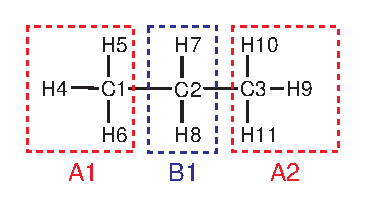
\includegraphics[width=6cm]{usage/fig/propane.eps}
  \caption{Atom labeling and mapping from an all-atom to a united atom representation of a propane molecule.
  \label{fig:propane_map}
}
\end{wrapfigure}

Each mapping file contains a {\em topology} of the coarse-grained molecule and a list of {\em maps}. Topology specifies coarse-grained beads and bonded interactions between them. Each coarse-grained bead has a name, type, a list of atoms which belong it, and a link to a map. A map is a \hyperref[sec:mapping_operator]{set of weights} $c_{Ii}$ for an atom $i$ belonging to the bead $I$. It is used to calculate the position of a coarse-grained bead from the positions of atoms which belong to it. Note that $c_{Ii}$ will be automatically re-normalized if their sum is not equal to 1, i.~e. in the case of a center-of-mass mapping one can simply specify atomic masses.
A complete reference for mapping file definitions can be found in sec.~\ref{sec:ref_mapping}.

As an example, we will describe here a mapping file of a united atom model of a propane molecule, chemical structure of which is shown in fig.~\ref{fig:intro:propane}. In this coarse-grained model two bead types (A,B) and three beads (A1, B1, A2) are defined, as shown in fig.~\ref{fig:propane_map}. We will use centers of mass of the beads as  coarse-grained coordinates.

Extracts from the \texttt{propane.xml} file of the tutorial are shown below. The \mapopt{name} tag provides the molecule name in the coarse-grained topology. The \mapopt{ident} tag must match the name of the molecule in the atomistic representation. In the \mapopt{topology} section all beads are defined by specifying bead name (A1, B1, A2), type, and atoms belonging to this bead in the form \texttt{residue id:residue name:atom name}. For each bead a map has to be specified, which is defined later in \mapopt{maps} section. Note that bead \hyperlink{\mapref{topology.cg_beads.cg_bead.type}}{type} and \hyperlink{\mapref{maps.map}}{map} can be different, which might be useful in a situation when chemically different beads (A1, B1) are assigned to the same bead type. After defining all beads the bonded interactions of the coarse-grained molecule must be specified in the \hyperlink{\mapref{topology.cg_bonded}}{cg\_bonded} section. This is done by using the identifiers of the beads in the coarse-grained model. Finally, in the \hyperlink{\mapref{topology.cg_beads.cg_bead.mapping}}{mapping} section, the mapping coefficients are defined. This includes a weighting of the atoms in the topology section. In particular, the number of weights given should match the number of beads.

\section{Verification of a mapping}
\label{sec:mapping_verification}
Note that the \mapopt{ident} tag should match the molecule name in the reference system. A common mistake is that beads have wrong names. In this case, the \prog{csg_dump} tool can be used in order to identify the atoms which are read in from a topology file *.tpr. This tool displays the atoms in the format \texttt{residue id:residue name:atom name}. For multicomponent systems, it might happen that molecules are not identified correctly. The workaround for this case is described in~\sect{sec:adv_topology}.

To compare coarse-grained and atomistic configurations one can use a standard visualization program, e.~g. \texttt{vmd}.  When comparing trajectories, one has to be careful, since \texttt{vmd} opens both a .gro and .trr file. The first frame is then the .gro file and the rest is taken from the .trr file. The coarse-grained trajectory contains only the frames of the  trajectory. Hence, the first frame of the atomistic run has to be removed using the \texttt{vmd} menu.


\begin{figure}
\centering
\framebox{
\lstinputlisting{functionality/propane.xml}
}
\caption{An extract from the mapping file \texttt{propane.xml} of a propane molecule. The complete file can be found in the \texttt{propane/single\_molecule} tutorial.}
\end{figure}

\section{Advanced topology handling}
\label{sec:adv_topology}
A topology is completely specified by a set of beads, their types, and a list of bonded interactions. \votca is able to read topologies in the \gromacs \texttt{.tpr} format. For example, one can create a coarse-grained topology based on the mapping file and atomistic \gromacs topology using \prog{csg_gmxtopol}.
\begin{verbatim}
  csg_gmxtopol --top topol.tpr --cg propane.xml --out out.top
\end{verbatim}


In some cases, however, one might want to use a .pdb file which does not contain all information about the atomistic topology. In this case, additional information can be supplied in the \xml mapping file.

A typical example is lack of a clear definition of molecules, which can be a problem for simulations with several molecules with multiple types. During coarse-graining, the molecule type is identified by a name tag as names must be clearly identified. To do this, it is possible to read a topology and then modify parts of it. The new \xml topology can be used with the \progopt{---tpr} option, as any other topology file.

For example, if information about a molecule is not present at all, one can create one from a \texttt{.pdb} file as follows
\begin{lstlisting}
<topology base="snapshot.pdb">
  <molecules>
    <clear/>
    <define name="mCP" first="1" nbeads="52" nmols="216"/>
  </molecules>
</topology>
\end{lstlisting}
where $<$clear/$>$ clears all information that was present before.

Old versions of \gromacs did not store molecule names. In order to use this feature, a recent \texttt{.tpr} file containing molecule names should always be provided. For old topologies, rerun \gromacs \progex{grompp} to update the old topology file.

If molecule information is already present in the parent topology but molecules are not named properly (as it is the case with old \gromacs \progopt{.tpr} files), one can rename them using
\begin{lstlisting}
 <topology base="topol.tpr">
   <molecules>
     <rename name="PPY3" range="1:125"/>
     <rename name="Cl" range="126:250"/>
   </molecules>
 </topology>
\end{lstlisting}
Here, the file \progopt{topol.tpr} is loaded first and all molecules are renamed afterwards.

\section{Trajectories}
\label{sec:trajectory}

A trajectory is a set of frames containing coordinates (velocities and forces) for the beads defined in the topology. \votca currently supports \texttt{.trr}, \texttt{.xtc}, \texttt{.pdb} and \texttt{.gro} trajectory formats.

Once the mapping file is created, it is easy to convert an atomistic to a coarse-grained trajectory using \prog{csg_map}
\begin{verbatim}
  csg_map --top topol.tpr --trj traj.trr --cg propane.xml --out cg.gro
\end{verbatim}

The program \prog{csg_map} also provides the option \progopt{---no-map}. In this case, no mapping is done and \prog{csg_map} works as a trajectory converter. In general, mapping can be enabled and disabled in most analysis tools, e.g. in \prog{csg_stat} or \prog{csg_fmatch}.

Note that the topology files can have a different contents as bonded interactions are not provided in all formats. In this case, mapping files can be used to define and relabel bonds.

Also note that the default setting concerning mapping varies individually between the programs. Some have a default setting that does mapping (such as \prog{csg_map}, use \progopt{---no-map} to disable mapping) and some have mapping disabled by default (e.g. \prog{csg_stat}, use \progopt{---cg} to enable mapping).

\section{Setting files}
\label{sec:setting_files}

\begin{figure}[h]
\centering
\begin{lstlisting}[frame=single]
<cg>
  <non-bonded> <!-- non-bonded interactions -->
    <name>A-A</name> <!-- name of the interaction -->
    <type1>A</type1> <!-- types involved in this interaction -->
    <type2>A</type2>
    <min>0</min>  <!-- dimension + grid spacing of tables-->
    <max>1.36</max>
    <step>0.01</step>
    <inverse>
      ... specific commands
    </inverse>

    ... specific section for inverse boltzmann, force matching etc.
  </non-bonded>
</cg>
\end{lstlisting}
\caption{Abstract of a \texttt{settings.xml} file. See sec. \ref{sec:preparing_the_run} for a full version.}
\end{figure}

A setting file is written in the format \texttt{.xml}. It consists of a general section displayed above, and a specific section depending on the program used for simulations. The setting displayed above is later extended in the sections on iterative boltzmann inversion (\prog{csg_inverse}), force matching (\prog{csg_fmatch}) or statistical analysis (\prog{csg_stat}).

Generally, \prog{csg_stat} is an analysis tool which can be used for computing radial distribution functions and analysing them. As an example, the command

\begin{verbatim}
  csg_stat --top topol.tpr --trj traj.xtc --options settings.xml
\end{verbatim}

computes the distributions of all interactions specified in \texttt{settings.xml} and writes all tabulated distributions as files \texttt{``interaction name''.dist.new}.

\section{Table formats}
\label{sec:table_formats}
Distribution functions, potentials and forces are returned as tables and saved in a file. Those tables generally have the format
\begin{verbatim}
  x y [error] flag
\end{verbatim}
where \texttt{x} is input quantity (e.g. radius $r$, angles $\theta$ or $\phi$), \texttt{y} is the computed quantity (e.g. a potential) and \texttt{[error]} is an optional error for \texttt{y}. The token \texttt{flag} can take the values \texttt{i}, \texttt{o} or \texttt{u}.
In the first case, \texttt{i} (\texttt{in range}) describes a value that lies within the data range, \texttt{o} (\texttt{out of range}) symbolises a value out of the data range and \texttt{u} stands for an \texttt{undefined} value.

The token \texttt{flag} will be important when extrapolating the table as described in sec. \ref{sec:post_processing}.
\chapter{Preparing coarse-grained runs}
\label{sec:usage:cgrun}

\subsection*{Preliminary note}
The coarse-grained run requires the molecule topology on the one hand and suitable potentials on the other. In this chapter, the generation of coarse-grained runs is decribed next, followed by a post-processing of the potential.

If the potential is of such a form that it allows direct fitting of a functional form, the section on post-processing can be skipped. Instead, a program of choice should be used to fit a functional form to the potential. Nevertheless, special attention should be paid to units (angles, bondlengths). The resulting curve can then be specified in the MD package used for simulation. However, most potentials don't allow an easy processing of this kind and tabulated potentials have to be used.

\section{Generating a topology file for a coarse-grained run}
\subsubsection*{WARNING: This section describes experimental features. The exact names and options of the program might change in the near future.  The section is specific to \gromacs support though a generalization for other MD packages is planned.}

The mapping definition is close to a topology needed for a coarse grained run. To avoid redundant work, \prog{csg_gmxtopol} can be used to automatically generate a gromacs topology based on an atomistic reference system and a mapping file.

At the current state, \prog{csg_gmxtopol} can only generate the topology for the first molecule in the system. If more molecule types are present, a special tpr file has to be prepared. The program can be executed by
\begin{verbatim}
  csg_gmxtopol --top topol.tpr --cg map.xml --out cgtop
\end{verbatim}
which will create a file \texttt{cgtop.top}. This file includes the topology for the first molecule including definitions for atoms, bonds, angles and dihedrals. It can directly be used as a topology in \gromacs, however the force field definitions (atom types, bond types, etc.) still have to be added manually.

\section{Post-processing of the potential}
\label{sec:post_processing}
The \votca package provides a collection of scripts to handle potentials. They can be modified, refined, integrated or inter- and extrapolated. These scripts are the same ones as those used for iterative methods in chapter \ref{sec:iterative_methods}. Scripts are called by \prog{csg_call}. A complete list of available scripts can be found in sec. \ref{sec:csg_table}.

The post-processing roughly consists of the following steps (see further explanations below):
\begin{itemize}
  \item (manually) clipping poorly sampled (border) regions
  \item resampling the potential in order to change the grid to the proper format (\prog{csg_resample})
  \item extrapolation of the potential at the borders (\prog{csg_call} table extrapolate)
  \item exporting the table to xvg (\prog{csg_call} convert\_potential xvg)
\end{itemize}

\subsection*{Clipping of poorly sampled regions}
Regions with an irregular distribution of samples should be deleted first. This is simply done by editing the \progopt{.pot} file and by deleting those values.

Alternatively, manually check the range where the potential still looks good and is not to noisy and set the flags in the potential file of the bad parts by hand to \texttt{o} (for \texttt{out of range}). Those values will later be extrapolated and overwritten.

\subsection*{Resampling}
Use the command
\begin{verbatim}
  csg_resample --in table.pot --out table_resample.pot \
               --grid min:step:max
\end{verbatim}
to resample the potential given in file --\progopt{table.pot} from \progopt{min} to \progopt{max} with a grid spacing of \progopt{step} steps. The result is written to the file specified by \progopt{out}. Additionally, \prog{csg_resample} allows the specification of spline interpolation (\progopt{spfit}), the calculation of derivatives (\progopt{derivative}) and comments (\progopt{comment}). Check the help (\progopt{help}) for further information.

It is important to note that the values \progopt{min} and \progopt{max} \textit{don't} correspond to the minimum and maximum value in the input file, but to the range of values the potential is desired to cover after extrapolation. Therefore, values in $[ \min,\max ]$ that are not covered in the file are automatically marked by a flag \texttt{o} (for \texttt{out of range}) for extrapolation in the next step.

\subsection*{Extrapolation}
The following line
\begin{verbatim}
  csg_call table extrapolate [options] table_resample.pot \
           table_extrapolate.pot
\end{verbatim}
calls the extrapolation procedure, which processes the range of values marked by \prog{csg_resample}. The input file is \progopt{table\_resample.pot} created in the last step.

After resampling, all values in the potential file that should be used as a basis for extrapolation are marked with an \texttt{i}, while all values that need extrapolation are marked by \texttt{o}. The command above now extrapolates all \texttt{o} values from the \texttt{i} values in the file. Available options include averaging over a certain number of points (\progopt{avgpoints}), changing the functional form (\progopt{function}, default is quadratic), extrapolating just the left or right region of the file (\progopt{region}) and setting the curvature (\progopt{curvature}).

The output \progopt{table\_extrapolate.pot} of the extrapolation step can now be used for the coarse-grained run. If \gromacs is used as a molecule dynamics package, the potential has to be converted and exported to a suitable \gromacs format as described in the final step.

\subsection*{Exporting the table}
Finally, the table is exported to \progopt{xvg}. The conversion procedure requires a small script \progopt{table.xml} as shown below:
\begin{verbatim}
  <cg>
    <inverse>
      <gromacs>
        <pot_max>1e8</pot_max>
        <table_end>8.0</table_end>
        <table_bins>0.002</table_bins>
      </gromacs>
    </inverse>
  </cg>
\end{verbatim}
where \progopt{<table\_end>} is the \gromacs \progopt{rvdw+table\_extension} and \progopt{<pot\_max>} is just a number slightly smaller than the upper value of single/ double precision. The value given in \progopt{<table\_bins>} corresponds to the \progopt{step} value of \progopt{csg\_resample -grid min:step:max}.

Using the \progopt{xml} file above, call
\begin{verbatim}
  csg_call --options table.xml convert_potential xvg \
           table_extrapolate.pot table.xvg
\end{verbatim}
to convert the extrapolated values in \progopt{table\_extrapolate.pot} to \progopt{table.xvg} (The file will contain \gromacs C12 parts only which are stored in the sixth und seventh column. Ensure compatibility with the \gromacs topology. See the \gromacs manual for further information).

To obtain a bonded table, run
\begin{verbatim}
  csg_call --options table.xml convert_potential xvg --type bonded \
           table_extrapolate.pot table.xvg
\end{verbatim}

\subsection*{An example on non-bonded interactions}
\begin{verbatim}
  csg_call pot shift_nb table.pot table.pot.refined
  csg_resample --grid 0:0.002:2 --in table.pot.refined \
           --out table.pot.refined
  csg_call table extrapolate --function quadratic --region left \
           table.pot.refined table.pot.refined
  csg_call table extrapolate --function constant --region right \
           table.pot.refined table.pot.refined
\end{verbatim}

%csg_call table integrate table.force table.pot (diese zeile nur bei force-matching)

\section{Alternatives}
Additionally to the two methods described above, namely (a) providing the MD package directly with a functional form fitted with a program of choice or (b) using \progopt{csg\_resample}, \progopt{csg\_call table extrapolate} and \progopt{csg\_call convert\_potential}, another method would be suitable. This is integrating the force table as follows
\begin{verbatim}
  -Integrate the table
  $csg_call table integrate force.d minus_pot.d
  -multiply by -1
  $csg_call table linearop minus_pot.d pot.d -1 0
\end{verbatim}

\chapter{Program usage}
\section{Boltzmann Inversion}
\begin{figure}
   \centering
   \includegraphics{usage/fig/flow_boltzmann.eps}
   \caption{Flowchart to perform Boltzmann inversion.}
\end{figure}

Boltzmann inversion is most often performed on a single molecule in vaccuum for deriving bonded interactions while the non-bonded parts are treated via a separate method. VOTCA offers tools to analyse distributions and correlations of such a simulation as well as the preparation of an tabulated potential. Also exclusion lists for the atomistic simulations when the separation ansatz is used (cite Tschoep) can be created automatically. The tool most often used in this section is \textbf{csg\_boltzmann}. Also mapping from atomistic to coarse-grained level can be perfomred. An important thing to remember if the program \textbf{csg\_boltzmann} is used is that it parses the whole trajectory and stores all information about bonded interactions in memory to allow interactive analysis. That's why it is not suitable for really big systems with lots of chains. If analysis of a big system is performed, \textbf{csg\_stat} should be prefered for the analysis. Though it currently offers less features than \textbf{csg\_boltzmann}, memory problems should not occur.

\subsection{Mapping scheme}
The first thing to coarse-grain a system is to define a mapping scheme (see \sect{sec:mapping}). The mapping is defined by a simple xml file for each molecule-type. An important step is to verify the mapping scheme by:

\begin{verbatim}
  csg_boltzmann --top topol.tpr --trj traj.trr --cg mapping.xml --out cg.gro
\end{verbatim}

The most common thing that can go wrong is that beads cannot be found. On reason is a type in the atom name of the mapping. To debug which atoms are read in from a topology file, \textbf{csg\_dump} can be used. A second reason could be, that molecules are not identified correctly. In case of a multicomponent system, see \sect{sec:adv_topology} for details.

In case everything works find, a file cg.gro which contains the coarse-grained trajectory is created. The easuiest way to compare coarse-grained and atomistic representation is to open both in e.g. vmd.  Be careful when opening in vmd specifying a .gro file + .trr, the first frame comes from the .gro, the following correspond to the trr. The coarse grained file only contains the frames from the trajectory, to compare them, the first frame of the atomistic run has to be deleted in vmd!!

\subsection{Generating reference trajectories with proper exclusions}
When the Boltzmann inversion method was described in Ref.\cite{Tschoep:1998}, bonded and non-bonded interactions were treated separately. To do this, a special atomistic trajectory is needed, where all non-bonded interactions are excluded which do not contribute to a bonde interaction in the coarse grained model. Manually this can be a complicated task, however textbf{csg\_boltzmann} offers the option \textbf{--excl} to do this automaticaly.

To generate an exclusion list automaticaly, an atomistic topology without exclusions and a mapping scheme has to be prepared first. Since VOTCA can currently only read GROMACS .tpr trajectories and not .top files, running \textbf{grompp} is obligatory. Important to note here is, that \textbf{csg\_boltzmann} currently only creates the exclusion list for the fist mulecule in the topology.

To create the exclusion list, run
\begin{verbatim}
  csg_boltzmann --top topol.tpr --cg mapping.xml --excl exclusions.txt
\end{verbatim}
This will create a list of exclusions for all interactions that are not within a bonded interaction of the coarse-grained sub-bead. As an example, if the coarse grained molecule is a linear molecule of 3 beads, which are only connected by bonds, \textbf{csg\_boltzmann} will create exclusions for all non-bonded interactions of atoms from the first bead with atoms of the 3rd bead since they would contribute only to the non-bonded interaction potential which is treated separately.

To add the exclusions to the gromacs topology of the molecule, either include the file specified in --excl as follows
\begin{verbatim}
  [ exclusions ]
  #include "exclusions.txt"
\end{verbatim}
or copy and paste the content of that file to the exclusions section.


\subsection{Analysis}
If the --trj option is specified to parse a reference trajectory, \textbf{csg\_boltzmann} enters an interactive mode which accepts commands.

\begin{verbatim}
  csg_boltzmann --top topol.top --trj traj.trr --cg mapping.xml 
\end{verbatim}

Here, analysis operations can be performed on all interactions evaluated. All interactions specified in the mapping schema are evaluated. A specific interaction is refered to by a name which is composed of \textit{molecule:interaction-group:index}, where molecule is the molecule number in the whole topology, interaction-group the name specified in the mapping file, and index the entry in the list of this interaction. E.g. \textit{1:AA-bond:10} is the 10th AA-bond in molecule 1. To show a list all interactions that where passed, the command \textit{list} can be used. To specify a couple of interactions during analysis, either give interactions separated by space of use wildcards (e.g. *:AA-bond*).

To quit interactive mode, use command \textit{q}. If analysis commands should be read from a file, use the pipe or stdin redirects from the shell.

\subsubsection{Distribution functions and tabulated potentials}
Distribution functions (tabulated potentials) can be created with the \textit{hist} (\textit{tab}) command.
To e.g. write out the distribution function for all interactions of group AA-bond (where AA-bond is the name specified in the mapping scheme) to file AA.txt, type
\begin{verbatim}
  hist AA.txt *:AA-bond:*   
\end{verbatim}
The command
\begin{verbatim}
  hist set
\end{verbatim}
prints a list of all parameters than can be changed for the histogram. To directly write the boltzmann inverted potential, the \textit{tab} command can be used. It's usage and options are very similar to the \textit{hist} command. If tabulated potentials are written, special care should be taken to the paramter T (temperature) and scale. The scale command does the volume normalization as given in     \eq{eq:boltzmann_norm}. Possible values are \textit{no} (no scaling), \textit{bond} (normalize for bonds) and \textit{angle} (normalize for angles). The e.g. write out the tabulated potential for an angle potential where the temperature was 300K type:
\begin{verbatim}
  tab set T 300
  tab set scale angle
  tab angle.pot *:angle:*
\end{verbatim}

\subsubsection{Correlation analysis}

\section{Force matching}
\sasha
\begin{figure}
   \centering
   \includegraphics{usage/fig/flow_fmatch.eps}
   \caption{Flowchart to perform force matching.}
\end{figure}
Force matching algorithm with cubic spline basis is implemented in \prog{csg_fmatch} utility.

\subsection{csg\_fmatch: available options}
When executing without any options \prog{csg_fmatch} shows available options:
\begin{verbatim}
  --options arg          options file for coarse graining
  --help                 produce this help message
  --version              show version info
  --top arg              atomistic topology file
  --trj arg              atomistic trajectory file
  --cg arg               coarse graining definitions (xml-file)
  --begin arg            skip frames before this time
  --first-frame arg (=0) start with this frame
  --nframes arg          process so many frames
\end{verbatim}
Some options must be provided, some are optional. Must be provided: \progopt{--options}, \progopt{--top}, \progopt{--trj} and \progopt{--cg}. \progopt{--top} is an atomistic topology file e.g. topol.tpr. \progopt{--trj} is an atomistic trajectory file: traj.trr. Note that trajectory file must contain forces ( there is an option for that in GROMACS .mdp file ), otherwise there will be nothing to match. \progopt{--cg} is a file, which contains the CG mapping scheme with all the interactions, user wants to define on a coarse-grained level, see \sect{sec:adv_topology}.

\subsubsection{CG-options file}
\progopt{--options} is an \xml-file, which contains options to control force matching functionality. 
Currently the file has the following options:

\begin{lstlisting}
   <cg>
     <!--fmatch section -->
     <fmatch>
       <!--Number of frames for block averaging -->
       <frames_per_block>6</frames_per_block>
       <!--Constrained least squares?-->
       <constrainedLS>false</constrainedLS>
     </fmatch>
     <!-- example for a non-bonded interaction entry -->
     <non-bonded>
       <!-- name of the interaction -->
       <name>CG-CG</name>
       <type1>A</type1>
       <type2>A</type2>
       <!-- fmatch specific stuff -->
       <fmatch>
         <min>0.27</min>
         <max>1.2</max>
         <step>0.02</step>
         <out_step>0.005</out_step>
       </fmatch>
     </non-bonded>
   </cg>
\end{lstlisting}

\textbf{frames\_per\_block}\newline is number of frames, being used for block averaging. Atomistic trajectory, specified with
\textbf{\ddash{trj}} option, is divided into blocks and the force matching equations are solved separately for each block.
Coarse-grained force-field, which one gets on the output is averaged over those blocks.

\textbf{constrainedLS}\newline is a boolean variable: false - simple least squares, true - constrained least squares. For details see \votca paper.
Practically both algorithms give the same results, but simple least squares is faster. If you are mathematician and think that a spline is only then can be called spline if it has continuous first and second derivatives, use constrained least squares. \newline

In this example we have only one interaction on a coarse-grained level, its name: CG-CG. But in principle several types of non-bonded as well as bonded interactions can be added. 

\textbf{type1} and \textbf{type2}\newline are the types of CG-beads involved in the interaction CG-CG. In this case this is an interaction between a CG-bead of type A with another CG-bead of type A. These types should correspond to the mapping scheme file ( option \progopt{--cg} ).
 
\textbf{min}\newline is a minimum distance between CG-bead of \textbf{type1} and CG-bead of \textbf{type2},  sampled in atomistic MD simulation. One can get this number by looking at the \textbf{type1-type2} radial distribution function. For CG bonds and angles the variable has the similar meaning ( note, that for angles it is specified in radians ).

\textbf{max}\newline is the interaction cutoff in case of non-bonded interaction or a maximum value, sampled in the atomistic simulations in case of bonded interactions.

\textbf{step}\newline is the grid spacing for the spline, which represents the interaction. This parameter should not be too big, otherwise you might lose some features of the interaction potential, and not too small, otherwise you will have unsampled bins and will get NaNs in the output.

\textbf{out\_step}\newline is a grid spacing for the output grid. Normally one wants to have this parameter smaller than \textbf{step}, 
to have smooth curve, without additional spline interpolation. 
As a rule of thumb we normally use \textbf{out\_step}, which is approximately 5 times smaller than \textbf{step}.

\subsection{Program output}
\prog{csg_fmatch} produces a separate .force file for each interaction, specified in the CG-options file (option \progopt{options} ).
These files have 4 columns: distance, corresponding force, table flag and the force error, estimated using block-averaging procedure.
If you have an angle, then the first column will contain corresponding angle in radians.

To get table-files for \gromacs one has to integrate the forces to get the potentials and do extrapolation and probably smoothing.

Output files are not only produced at the end of the program execution, but after successfull processing of every block. The user can have a look at the output files and decide to stop \prog{csg_fmatch}, as long as the force error is small enough.

\subsection{Integration and extrapolation of .force files }
To convert .force to .pot one can execute

\begin{verbatim}
 csg_call table integrate CG-CG.force CG-CG.pot
\end{verbatim}

This command calls {\it integrate.pl} script, which integrates the force and writes the potential to the .pot file.

Normally, some range of distances is not sampled in atomistic simulations. For example, very small distances are never sampled in the case of non-bonded interactions. But you might want to have them in your \gromacs table. So you have to extrapolate your potential. In order to do this one has to resample the grid first:

\begin{verbatim}
 csg_resample --in CH2-CH2.pot --out CH2-CH2.resampled.pot --grid 0:0.001:1.4
\end{verbatim}

Finally you can call {\it extrapolate.pl } to extrapolate the potential, for example:

\begin{verbatim}
 csg_call table extrapolate --function linear 
--region leftright CH2-CH2.resampled.pot CH2-CH2.extrapolated.pot
\end{verbatim}






\section{Iterative Boltzmann Inverse}
\begin{figure}
   \centering
   \includegraphics{usage/fig/flow_ibi.eps}
   \caption{\label{fig:flow_ibi}Flowchart to perform iterative Boltzmann inversion.}
\end{figure}

\subsection{Input preparation}
In this section, the usage of \ibi is described which is implemented within the scripting framework described in \sect{sec:impl:scripting}. It is suggested to get a basic understaning of this framework before proceeding.

\ibi so far only supports iterative refinement of non-bonded interactions. An outline of the workflow for performing \ibi is given in \fig{fig:flow_ibi}. The first thing to do is generate reference distribution functions. These might come from experiments or from atomistic simulations. To get reasonable results out of the iterative process, the reference distributions should be of good quality (little noise, etc).

\votca can create initial guesses for the coarse-grained potentials by boltzmann inverting the distribution function. If a custom initial guess for an interaction needs to be used instead, the table can be provided in \textit{$<$interaction$>$.pot.in}. As already mentioned, \votca automatically creates potential tables to run a simulation. However it does not know how to run a coarse-grained simulation. Therefore, all files needed to run a coarse-grained simulation, except for the potentials that are iteratively refined, must be provided and added to the \hyperlink{\cgref{inverse.filelist}}{filelist} in the settings \xml-file. If an atomistic topology and a mapping definition are present, \votca offers tools to assist the setup of a  coarse-grined topology (see \sect{sec:usage:cgrun}).

To get an overview of how an input file for doing \ibi looks like, it is suggested to take a look at one of the tutorials provided on \votcaweb.

\subsection{Pressure correction}

The pressure of the coarse-grained system usually does not match the pressure of the full atomistic system. The reason is that during the itereative boltzmann inversion only structural properties and not thermodynamic properties are targeted. In order correct the pressure to match the target pressure, different strategies have been used based on small modifications of the potential. The correction can be applied via \interopt{post_update} scripts. The type of pressure correction is selected as described in section \sect{sec:ref_interaction}.


\subsubsection{Simple pressure correction}
In ref.\cite{Reith:2003} a simple linear attractive potential was added to the coarse-grained potential
\begin{equation}
  \Delta V(r)=A(1-\frac{r}{r_{cutoff}}) \,.
\end{equation}
with prefactor $A$
\begin{equation}
  A = -\operatorname{sgn}(\Delta P)0.1k_{B}T\min(1,|f\Delta P) \,,
\end{equation}
$\Delta p=P_i-P_{target}$, and the scaling factor f which can be specified in the settings file.

An example for a block to do simple pressure correction every third interaction is
\begin{lstlisting}
<post_update>pressure</post_update>
<post_update_options>
  <pressure>
    <type>simple</type>
    <do>0 0 1</do>
    <simple>
      <scale>0.0003</scale>
    </simple>
  </pressure
</post_update_options>
\end{lstlisting}
Here, \interopt{inverse.post_update_options.pressure.simple.scale} is the scaling factor $f$. In order to get the correct pressure it can become necessary to tune the scaling factor $f$ during the iterative process.

\subsubsection{Advanced pressure correction}
In \cite{Wang:2009} a pressure correction based on the virial expression of the pressure was introduced. The potential term is the same as in the simple form with a different form of the $A$ factor being used:
\begin{equation}
  A = \left[\frac{-2\pi\rho^{2}}{3r_{cut}}\int_{0}^{r_{cut}}r^{3}g_{i}(r)dr\right]A_{i}=\Delta P
\end{equation}
This requires as an additional input parameter the particle density $ \rho $ to be provided, which is added as  \interopt{inverse.particle density} in the input file. 

\subsection{Runtime optimization}
Most of the time for each iteration is spent in running the coarse-grained system and calculate the statistics. To get a feeling on how much statistics is needed, it is recommended to plot the distribution functions and check whether they are sufficiently smooth. Bad statistics lead to rough potential updates and the iterative refinement might fail. The runs should be long enough to produce distributions/rdfs with reasonable quality.

Often, runtime can be improved by smoothing the potential updates. Our experience has shown that it is better to smooth the potential update instead of the rdf or potential itself. If the potential or rdf is smoothed, sharp features like the first peak in \spce water might get lost. Smoothing on the delta potential works quite well, since the sharp features are already present from the initial guess. By applying iterations of a simple triangular smoothing ($ \Delta U_i = 0.25 \Delta U_{i-1} + 0.5\Delta U_i + 0.25\Delta U_{i+1} $), a reasonable coarse-grained potential for \spce water could be produced in less than 10 minutes. Smoothing is implemented as a post\_update script and can be enabled by adding
\begin{lstlisting}
  <post_update>smooth</post_update>
  <post_update_options>
    <smooth>
        <iterations>2</iterations>
    </smooth>
  </post_update_options>
\end{lstlisting}
to the inverse section of an interaction in settings \xml.




\chapter{Inverse Monte Carlo}
In this section, additional options are described to run \imc coarse graining. The usage of imc is similar to \ibi, it is necessary to understand the use of the scripting framework described in chapter~\ref{sec:iterative_workflow}.

\textbf{WARNING: multicomponent \imc is still experimental!}

\section{General considerations}
In comparison to \ibi, \imc needs a significant amount more statistics to calculate the potential update\cite{Ruehle:2009.a}. It is advisable to perform smoothing on the potentual update. Smoothing can can be performed as described in \sect{ref:ibi:optimize}. In addition, \imc can lead to problems with finite size. For methanol, it was shown, that a too small system leads to a linear shift in the potential\cite{Ruehle:2009.a}. Always check, that the system size is sufficient and runlengh csg smoothing iterations is well balanced.

\section{Additional mapping for statistics}
The program \prog{csg_stat} is used for evaluating the \imc matrix. Although here it only acts on the coarse-grained system, it still needs a mapping file to work. This will change with one of the next releases to simplify the setup. The mapping file needs to be a one to one mapping of the coarse grained system, e.g. for coarse graining \spce water, the mapping file looks like the following.
\begin{lstlisting}
  </cg_molecule>
    <name>SOL</name> 
    <ident>SOL</ident>
    <topology>
      <cg_beads>
        <cg_bead>
          <name>CG</name>
          <type>CG</type>
          <mapping>A</mapping>
          <beads>
            1:SOL:CG 
          </beads>
        </cg_bead>
      </cg_beads>
    </topology>
    <maps>
      <map>
        <name>A</name>
        <weights>1</weights>
      </map>
    </maps>
  </cg_molecule>
\end{lstlisting}



\section{Correlation groups}
Unlike in \ibi, \imc also takes into account cross-correlations of interactions to calculate the update. However, it might not always be beneficial to evaluate cross-correlations of all pairs of interactions. By specifying \interopt{imc.group}, \votca allows to define groups of interactions, amongst which cross-correlations are taken into account, where \interopt{imc.group} can be any name.

\begin{lstlisting}
  <non-bonded>
    <name>CG-CG</name>
    <type1>CG</type1>
    <type2>CG</type2>
    ...
    <imc>
      <group>solvent</group>
   </imc>
  </non-bonded>
  <non-bonded>
\end{lstlisting}

\chapter{Preparing coarse-grained runs}
\label{sec:usage:cgrun}

\subsection*{Preliminary note}
The coarse-grained run requires the molecule topology on the one hand and suitable potentials on the other. In this chapter, the generation of coarse-grained runs is decribed next, followed by a post-processing of the potential.

If the potential is of such a form that it allows direct fitting of a functional form, the section on post-processing can be skipped. Instead, a program of choice should be used to fit a functional form to the potential. Nevertheless, special attention should be paid to units (angles, bondlengths). The resulting curve can then be specified in the MD package used for simulation. However, most potentials don't allow an easy processing of this kind and tabulated potentials have to be used.

\section{Generating a topology file for a coarse-grained run}
\subsubsection*{WARNING: This section describes experimental features. The exact names and options of the program might change in the near future.  The section is specific to \gromacs support though a generalization for other MD packages is planned.}

The mapping definition is close to a topology needed for a coarse grained run. To avoid redundant work, \prog{csg_gmxtopol} can be used to automatically generate a gromacs topology based on an atomistic reference system and a mapping file.

At the current state, \prog{csg_gmxtopol} can only generate the topology for the first molecule in the system. If more molecule types are present, a special tpr file has to be prepared. The program can be executed by
\begin{verbatim}
  csg_gmxtopol --top topol.tpr --cg map.xml --out cgtop
\end{verbatim}
which will create a file \texttt{cgtop.top}. This file includes the topology for the first molecule including definitions for atoms, bonds, angles and dihedrals. It can directly be used as a topology in \gromacs, however the force field definitions (atom types, bond types, etc.) still have to be added manually.

\section{Post-processing of the potential}
\label{sec:post_processing}
The \votca package provides a collection of scripts to handle potentials. They can be modified, refined, integrated or inter- and extrapolated. These scripts are the same ones as those used for iterative methods in chapter \ref{sec:iterative_methods}. Scripts are called by \prog{csg_call}. A complete list of available scripts can be found in sec. \ref{sec:csg_table}.

The post-processing roughly consists of the following steps (see further explanations below):
\begin{itemize}
  \item (manually) clipping poorly sampled (border) regions
  \item resampling the potential in order to change the grid to the proper format (\prog{csg_resample})
  \item extrapolation of the potential at the borders (\prog{csg_call} table extrapolate)
  \item exporting the table to xvg (\prog{csg_call} convert\_potential xvg)
\end{itemize}

\subsection*{Clipping of poorly sampled regions}
Regions with an irregular distribution of samples should be deleted first. This is simply done by editing the \progopt{.pot} file and by deleting those values.

Alternatively, manually check the range where the potential still looks good and is not to noisy and set the flags in the potential file of the bad parts by hand to \texttt{o} (for \texttt{out of range}). Those values will later be extrapolated and overwritten.

\subsection*{Resampling}
Use the command
\begin{verbatim}
  csg_resample --in table.pot --out table_resample.pot \
               --grid min:step:max
\end{verbatim}
to resample the potential given in file --\progopt{table.pot} from \progopt{min} to \progopt{max} with a grid spacing of \progopt{step} steps. The result is written to the file specified by \progopt{out}. Additionally, \prog{csg_resample} allows the specification of spline interpolation (\progopt{spfit}), the calculation of derivatives (\progopt{derivative}) and comments (\progopt{comment}). Check the help (\progopt{help}) for further information.

It is important to note that the values \progopt{min} and \progopt{max} \textit{don't} correspond to the minimum and maximum value in the input file, but to the range of values the potential is desired to cover after extrapolation. Therefore, values in $[ \min,\max ]$ that are not covered in the file are automatically marked by a flag \texttt{o} (for \texttt{out of range}) for extrapolation in the next step.

\subsection*{Extrapolation}
The following line
\begin{verbatim}
  csg_call table extrapolate [options] table_resample.pot \
           table_extrapolate.pot
\end{verbatim}
calls the extrapolation procedure, which processes the range of values marked by \prog{csg_resample}. The input file is \progopt{table\_resample.pot} created in the last step.

After resampling, all values in the potential file that should be used as a basis for extrapolation are marked with an \texttt{i}, while all values that need extrapolation are marked by \texttt{o}. The command above now extrapolates all \texttt{o} values from the \texttt{i} values in the file. Available options include averaging over a certain number of points (\progopt{avgpoints}), changing the functional form (\progopt{function}, default is quadratic), extrapolating just the left or right region of the file (\progopt{region}) and setting the curvature (\progopt{curvature}).

The output \progopt{table\_extrapolate.pot} of the extrapolation step can now be used for the coarse-grained run. If \gromacs is used as a molecule dynamics package, the potential has to be converted and exported to a suitable \gromacs format as described in the final step.

\subsection*{Exporting the table}
Finally, the table is exported to \progopt{xvg}. The conversion procedure requires a small script \progopt{table.xml} as shown below:
\begin{verbatim}
  <cg>
    <inverse>
      <gromacs>
        <pot_max>1e8</pot_max>
        <table_end>8.0</table_end>
        <table_bins>0.002</table_bins>
      </gromacs>
    </inverse>
  </cg>
\end{verbatim}
where \progopt{<table\_end>} is the \gromacs \progopt{rvdw+table\_extension} and \progopt{<pot\_max>} is just a number slightly smaller than the upper value of single/ double precision. The value given in \progopt{<table\_bins>} corresponds to the \progopt{step} value of \progopt{csg\_resample -grid min:step:max}.

Using the \progopt{xml} file above, call
\begin{verbatim}
  csg_call --options table.xml convert_potential xvg \
           table_extrapolate.pot table.xvg
\end{verbatim}
to convert the extrapolated values in \progopt{table\_extrapolate.pot} to \progopt{table.xvg} (The file will contain \gromacs C12 parts only which are stored in the sixth und seventh column. Ensure compatibility with the \gromacs topology. See the \gromacs manual for further information).

To obtain a bonded table, run
\begin{verbatim}
  csg_call --options table.xml convert_potential xvg --type bonded \
           table_extrapolate.pot table.xvg
\end{verbatim}

\subsection*{An example on non-bonded interactions}
\begin{verbatim}
  csg_call pot shift_nb table.pot table.pot.refined
  csg_resample --grid 0:0.002:2 --in table.pot.refined \
           --out table.pot.refined
  csg_call table extrapolate --function quadratic --region left \
           table.pot.refined table.pot.refined
  csg_call table extrapolate --function constant --region right \
           table.pot.refined table.pot.refined
\end{verbatim}

%csg_call table integrate table.force table.pot (diese zeile nur bei force-matching)

\section{Alternatives}
Additionally to the two methods described above, namely (a) providing the MD package directly with a functional form fitted with a program of choice or (b) using \progopt{csg\_resample}, \progopt{csg\_call table extrapolate} and \progopt{csg\_call convert\_potential}, another method would be suitable. This is integrating the force table as follows
\begin{verbatim}
  -Integrate the table
  $csg_call table integrate force.d minus_pot.d
  -multiply by -1
  $csg_call table linearop minus_pot.d pot.d -1 0
\end{verbatim}



\chapter{Advanced topics}
\label{sec:advanced_topics}

\section{Customization}
Each sub-step of an iteration and all direct calls can be adjusted to the user needs. The internal part of the iterative framework is organized as follows: all scripts are called using two keywords
\begin{verbatim}
  csg_call key1 key2
\end{verbatim}
For example, \texttt{csg\_call update imc} calls the \texttt{update} script for the inverse Monte Carlo procedure. The corresponding keywords are listed in \sect{sec:csg_table} or can be output directly by calling
\begin{verbatim}
  csg_call --list
\end{verbatim}

It is advised not to change already implemented scripts. To customize a script or add a new one, copy the script to your own directory (set by \cgopt{inverse.scriptpath}) and redirect its call by creating your own \texttt{csg\_table} file in this directory which looks like this
\begin{verbatim}
  key1 key2 script1 options
  key3 key4 script2
\end{verbatim}
If the local keys are already in use, the existing call will be overloaded.

As an example, we will illustrate how to overload the script which calls the sampling package. 
ohe \prog{csg_inverse} script runs \progex{mdrun} from the \gromacs package only on one cpu. Our task will be to change the script so that \gromacs uses 8 cpus, which is basically the same as adding mpirun options in \cgopt{inverse.gromacs.mdrun.command}.

First we find out which script calls \progex{mdrun}:
\begin{verbatim}
  csg_call --list | grep gromacs
\end{verbatim}
The output should look as follows
\begin{verbatim}
  init gromacs initalize_gromacs.sh
  prepare gromacs prepare_gromacs.sh
  run gromacs run_gromacs.sh
  pressure gromacs calc_pressure_gromacs.sh
  rdf gromacs calc_rdf_gromacs.sh
  imc_stat gromacs imc_stat_generic.sh
  convert_potential gromacs potential_to_gromacs.sh
\end{verbatim}
the third line indicates the script we need. If the output of \prog{csg_call} is not clear, one can try to find the right script in \sect{sec:csg_table}. Alternatively, check the folder
\begin{verbatim}
  <csg-installation>/share/scripts/inverse
\end{verbatim}
for all available scripts. 

Analyzing the output of
\begin{verbatim}
  csg_call --cat run gromacs
\end{verbatim}
we can conclude that this is indeed the script we need:
%
\begin{verbatim}
  USES: run_or_exit mdrun
  run_or_exit mdrun
\end{verbatim}
Now we can create our own \texttt{SCRIPTDIR}, add a new script there, make it executable and overload the call of the script:
\begin{verbatim}
  mkdir -p SCRIPTDIR
  cp `csg_call --quiet --show run gromacs` SCRIPTDIR/my_run_gromacs.sh
  chmod 755 SCRIPTDIR/my_run_gromacs.sh
  echo "run gromacs my_run_gromacs.sh" >> SCRIPTDIR/csg_table
\end{verbatim}
Please note that \texttt{my\_run\_gromacs.sh} is the name of the script and \texttt{SCRIPTDIR} is the custom script directory, which can be a global or a local path.
Now we change the last line of \texttt{my\_run\_gromacs.sh} to:
\begin{verbatim}
  run_or_exit mpirun -np 8 mdrun
\end{verbatim}
This completes the customization. Do not forget to add \texttt{SCRIPTDIR} to \cgopt{inverse.scriptpath} in the setting \xml file (see \sect{sec:ref_options}).

You can check the new script by running:
\begin{verbatim}
  csg_call --scriptdir SCRIPTDIR --list
  csg_call --scriptdir SCRIPTDIR --run run gromacs
\end{verbatim}

Finally, do not forget to remove the license infomation and change the version number of the script.

\section{Used external packages}

\subsection{GroMaCS}
\label{progpack.gromacs}
Get it from \htmladdnormallink{www.gromacs.org}{http://www.gromacs.org}
\begin{itemize}
\item \hypertarget{progex.mdrun}{\textbf{mdrun}}
\item \hypertarget{progex.grompp}{\textbf{grompp}}
\end{itemize}

\subsection{ESPResSo}
\label{progpack.espresso}
Get it from \htmladdnormallink{www.espressomd.org}{http://www.espressomd.org}

\subsection{Gnuplot}
\label{progpack.gnuplot}
Get it from \htmladdnormallink{www.gnuplot.info}{http://www.gnuplot.info}

\subsection{GNU Octave}
\label{progpack.octave}
Get it from \htmladdnormallink{www.gnu.org}{http://www.gnu.org/software/octave/}

\subsection{Matlab}
\label{progpack.matlab}
Get it from \htmladdnormallink{www.mathworks.com}{http://www.mathworks.com/products/matlab/}

\subsection{NumPy}
\label{progpack.numpy}
Get it from \htmladdnormallink{http://numpy.scipy.org}{http://numpy.scipy.org}

\chapter{Reference}
\section{Programs}
\label{sec:ref_programs}
\input{reference/programs/all}
\section{Mapping file}
\label{sec:ref_mapping}
The root node always has to be cg\_molecule. It can contain the following keywords:

\section{Mapping definitions}
{\em Mapping definitions} describe how to map a single molecule from atomistic to coarse-grained representation. The mapping definition have only to be specified once per molecule. The file contains sections for coarse-grained beads, bonded interactions in coarse grained scheme as well as mapping matrices. 

\subsection{Structure of mapping file}
The root node always has to be cg\_molecule. It can contain the following keywords:


\begin{itemize}
\item \textbf{ident} \\
      Molecule name in reference topology.
\item \textbf{maps} \\
      Section containing definitions of mapping schemes.
\item \textbf{maps.map} \\
      Section for a mapping for 1 bead.
\item \textbf{maps.map.name} \\
      Name of the mapping.
\item \textbf{maps.map.weights} \\
      Weights of the mapping matrix. Entries are normalized to 1, number of entries must match the number of reference beads in a coarse-grained bead.
\item \textbf{name} \\
      Name of molecule in coarse-grained representation.
\item \textbf{topology} \\
      Section containing definition of coarse grained topology of molecule.
\item \textbf{topology.cg\_beads} \\
      Section defining coarse grained beads of molecule.
\item \textbf{topology.cg\_beads.cg\_bead} \\
      Definition of a coarse grained bead.
\item \textbf{topology.cg\_beads.cg\_bead.beads} \\
      The beads section lists all atoms of the reference system that are mapped to this particular
      coarse grained bead. The syntax is RESID:RESNAME:ATOMNAME, the beads are seperated by spaces.
\item \textbf{topology.cg\_beads.cg\_bead.mapping} \\
      Mapping scheme to be used for this bead (specified in section mapping) to map from reference system.
\item \textbf{topology.cg\_beads.cg\_bead.name} \\
      Name of coarse grained bead.
\item \textbf{topology.cg\_beads.cg\_bead.type} \\
      Type of coarse grained bead.
\item \textbf{topology.cg\_bonded} \\
      The cg\_bonded section contains all bonded interaction of the molecule. That can be bond, angle or dihedral.
      An entry for each group of bonded interaction can be specified, e.g. several groups (types) of bonds can be specified.
      A specific bonded interaction can be later on addressed by MOLECULE:NAME:NUMBER, where MOLECULE is the molecule ID in
      the whole topology, NAME the name of the interaction group and NUMBER addresses the interaction in the group.
\item \textbf{topology.cg\_bonded.angle} \\
      Definition of a group of angles.
\item \textbf{topology.cg\_bonded.angle.beads} \\
      List of triples of beads that define a bond. Names specified in cg\_beads, separated by commas.
\item \textbf{topology.cg\_bonded.angle.name} \\
      Name of the group.
\item \textbf{topology.cg\_bonded.bond} \\
      Definition of a group of bonds.
\item \textbf{topology.cg\_bonded.bond.beads} \\
      List of pair of beads that define a bond. Names specified in cg\_beads, separated by commas.
\item \textbf{topology.cg\_bonded.bond.name} \\
      Name of the group.
\item \textbf{topology.cg\_bonded.dihedral} \\
      Definition of a group of dihedrals. Since the exact functional form does not matter, this combines proper as well as improper dihedrals.
\item \textbf{topology.cg\_bonded.dihedral.beads} \\
      List of quadruples of beads that define a bond. Names specified in cg\_beads, separated by commas.
\item \textbf{topology.cg\_bonded.dihedral.name} \\
      Name of the group.
\end{itemize}


\subsection{Example - mapping file for propane}

\lstinputlisting[frame=single,caption=Mapping for propane]{usage/propane.xml}


\section{Topology file}
\label{sec:ref_topology}
The \xml topology file

\input{reference/xml/topol.xml}

\section{Settings file}
All options for the iterative script are stored in an xml file.
\label{sec:ref_options}
\input{reference/xml/csg_defaults.xml}
\vfill

\section{Scripts}
\label{sec:csg_table}
Scripts are used by \prog{csg_call} and \prog{csg_inverse}.
The script table commonly used (compare \texttt{csg\_call --list}): 
\input{reference/scripts/csg_table}
Script calls can be overwritten by adding a line with the 3rd column changed to \texttt{csg\_table} in \cgopt{inverse.scriptpath} directory.
%\input{reference/scripts/all}


\bibliographystyle{unsrt}
\bibliography{votca}

\end{document} 
